%!TEX root = ../main.tex
\section{Human-in-the-loop Techniques for Machine Learning}
\label{sec:overview}

As shown in Section~\ref{sec:intro}, humans are involved frequently and necessarily in a machine learning pipeline.  They can not only contribute to the data preprocessing steps, but also  provide a large amount of labeled training data to build a well-performed machine learning  model, especially for the deep learning~\cite{DBLP:imagenet}. No matter what roles humans play in a ML pipeline, there exist some common sophisticated techniques to apply. In this section, we summarize some significant techniques in human involved machine learning. First, when humans are asked to conduct data annotation or data preprocessing, they are always required to provide high quality results, so we should study how to improve the quality of human answers in section~\ref{subsec:quality}. Second, since humans are not free, we study how to save monetary cost while not sacrificing much quality in section ~\ref{subsec:cost}. Third, since humans cannot perform as quickly as machines, latency should be reduced to accelerate the entire ML process(section~\ref{subsec:latency}).  Besides, active learning(section~\ref{subsec:active_learning}) focuses on selecting the most interesting examples to human for labeling to improve the model iteratively, which is an advanced technique in the field of machine learning. Lastly, in section \ref{subsec:weak}, we discuss the situation where the user cannot derive a number of high quality labels, so she has to use weak supervision techniques to build a model based on  weak labels, still with satisfying performance.
%Lastly, some recent works have focused on  leveraging human to label for the performance of the downstream ML application directly, which will be discussed in section ~\ref{subsec:downstream}.

\subsection{Quality Improvement}\label{subsec:quality}

Human answers may not be reliable because (1) there exist malicious humans that randomly return answers, especially in the crowdsourcing scenario and (2) some tasks are difficult for humans to answer. Therefore, it is significant to discover different characteristics of humans and tasks, which can be leveraged to improve the quality.  There are two commonly-used  techniques for quality improvement, i.e., truth inference and task assignment, which will be introduced as follows.


\textbf{Truth Inference.}
To control the quality, an intuitive idea is to assign each task to multiple humans, aggregate the answers and infer the truth. 
Note that humans may provide low quality or even malicious answers because they  may also have different levels of expertise, and an untrained human may be incapable of answering certain tasks. Therefore, to achieve high quality, we need to tolerate human errors and infer high-quality results from noisy answers. 

A unified quality control framework consists of the following three steps. First, we initialize each human's quality. Second, we infer the truth based on the collected answers and current quality. Third,  we estimate the quality according to the inferred truth. Then we iterate the second and third steps until converge. Based on the unified framework, existing works ~\cite{DBLP:faitcrowd, DBLP:conf/nips/WhitehillRWBM09} can be categorized based on the following three factors: task modeling, human modeling and applied techniques(how to use task and human modeling to infer the truth).

\textit{(1) Task Modeling.} This describes how existing solutions model a task, mainly including the difficulty of a task and the latent topics in a task~\cite{DBLP:faitcrowd, DBLP:conf/nips/WhitehillRWBM09}. First, some recent works model the difficulty levels of a task instead of assuming that a human has the same quality for answering all the tasks. The more difficult a task, the harder a human can provide a perfect answer for it. 
For example, in ~\cite{DBLP:conf/nips/WhitehillRWBM09}, $Pr(v_i^w = v_i^* | d_i, q^w) = 1/(1+ e^ {-d_i \cdot q^w} )$ denotes the probability that human $w$ correctly answers task $t_i$, where $d_i \in (0, + \infty)$ represents the difficulty of task $t_i$, $v_i^w$ is the worker's answer for a task $v_i$ whose true answer is $v_i*$, $q_w$ is the worker quality. The higher $d_i$, the easier task the $t_i$ . Intuitively, for a fixed human quality $q^w > $0, an easier task (high value of $d_i$) leads to a higher probability that the human correctly answers the task.
Second, some recent works model the difficulty as a vector with $K$ values instead of a single value.  The basic idea is to exploit diverse topics of a task, where $K$ is the pre-defined number of topics. For example, existing works ~\cite{DBLP:icrowd,DBLP:faitcrowd} apply topic model techniques on text description of each task to derive the topic vector. Besides, entity linking techniques are utilized to infer the  topic vector for each task~\cite{DBLP:docs}.


\textit{(2) Human Modeling.} This  describes how existing works model a human's quality, which is always denoted as a single real number $q^w \in [0,1]$, representing the probability that human $w$ answers a task correctly. This straightforward model has been widely adopted by existing works~\cite{DBLP:conf/nips/LiuPI12, DBLP:zencrowd, DBLP:conf/aaai/AydinYLLGD14}. More specifically, for single-choice tasks, existing works~\cite{DBLP:conf/www/VenanziGKKS14, DBLP:journals/jmlr/KimG12, raykar2010learning} extend the above model to the confusion matrix to model the human quality in a more fine-grained way. Suppose each task in  has $l$ fixed choices, then the confusion matrix $q^w$ is an $l × l$ matrix, where  the $j$-th ($1 \leq j \leq l$) row, i.e., $q^w_j = [ q^w_{j,1},q^w_{j,2},...,q^w_{j,l} ]$, represents the probability distribution of human w’s possible answers for a task if the truth of the task is the $j$-th choice. Each element $q^w_{j,k}$  denotes that given the truth of a task is the $j$-th choice, the probability that human $w$ selects the $k$-th choice. For numeric tasks, human bias and variance are proposed to model the human quality~\cite{raykar2010learning, welinder2010multidimensional}. Bias measures the effect that a human may underestimate (or overestimate) the truth of a task and variance measures the variation of errors around the bias. 
What's more, existing works \cite{DBLP:conf/kdd/JoglekarGP13, DBLP:journals/pvldb/LiLGSZDFH14} introduce confidence in quality control, i.e.,  if a human answers many
tasks, then the estimated quality for her is of high confident; otherwise the estimated quality is not confident. Inspired by this
, \cite{DBLP:journals/pvldb/LiLGSZDFH14} assigns higher qualities to the humans who answer plenty of tasks. 

\textit{(3) Applied Techniques.} In this part, we discuss how existing works leverage task models and human models to solve the truth inference problem. In general, existing works adopt the aforementioned unified framework, which can be categorized as the following three classes:  straightforward computation ~\cite{DBLP:conf/sigmod/FranklinKKRX11, DBLP:conf/cikm/ParameswaranPGPW12}, optimization methods~\cite{DBLP:conf/aaai/AydinYLLGD14, DBLP:journals/pvldb/LiLGSZDFH14, DBLP:conf/sigmod/LiLGZFH14, DBLP:conf/nips/ZhouPBM12} and probabilistic graphical model methods~\cite{DBLP:conf/nips/KargerOS11, DBLP:conf/nips/LiuPI12}. First,  the straightforward computation are some baseline models that estimate the truth without modeling the human or tasks. For single-label tasks, they always use the majority voting to address. For numerical tasks,  mean and median are two baseline methods that regard the mean and median of humans’ answers as the truth.  
Second, optimization methods focus on designing optimization functions that capture the relations between humans’ qualities and tasks’ truth, and then provide an iterative method to compute these two sets of parameters. The differences among existing works ~\cite{DBLP:conf/aaai/AydinYLLGD14, DBLP:journals/pvldb/LiLGSZDFH14, DBLP:conf/sigmod/LiLGZFH14, DBLP:conf/nips/ZhouPBM12} are that they model humans’ qualities based on the above human modeling part differently. 
Third,  probabilistic graph models a human’s quality as a node and utilize graphical model inference  to iteratively derive humans’ models~\cite{DBLP:conf/nips/KargerOS11, DBLP:conf/nips/LiuPI12}, where a graphical model is a graph, containing nodes and edges between pairs of nodes. Each node represents a random variable, which can be unknown parameters or observed data, and each edge represents the possible relationship (e.g., conditional dependency) between the linked pair of nodes. 


\textbf{Task Assignment.} \label{subsec:task_assignment}
 Since humans  diverse backgrounds and  qualities on tasks, a sophisticated task assignment algorithm will judiciously select  tasks to right humans. Existing works mainly focus on two  scenarios: (1) human-based, i.e., given a task, which subset of humans should be selected to answer the task; (2) task-based, i.e., when a human comes, which subset of tasks should be assigned to the human.
 
 \textit{(1) Human-based.}
 In this scenario, given a task and a set of candidate humans, the focus is on studying which subset of humans should be selected to answer the task in order to maximize the task’s quality without exceeding the overall budget. The problem is often called the “Jury Selection Problem” ~\cite{DBLP:journals/pvldb/CaoSTC12, DBLP:conf/edbt/ZhengCMM15}. Intuitively, humans with high quality should be selected.  To this end, Cao et al. [9] provide a framework that first studies how to compute the quality of a given subset of humans before they give  answers, called Jury Quality (JQ).  Since the answers are unknown in advance,  all possible cases of humans’ answers should be considered to compute the quality. To address this, Cao et al. ~\cite{DBLP:journals/pvldb/CaoSTC12} propose  a Majority Voting strategy to compute the JQ. Zheng et al. ~\cite{DBLP:conf/edbt/ZhengCMM15} prove that Bayesian Voting is the optimal strategy under the definition of JQ. That is, given any fixed subset of humans $S$, the JQ of $S$ w.r.t. the Bayesian Voting strategy is not lower than the JQ of S w.r.t. any other strategy. Therefore,  given a set of humans, its JQ w.r.t. Bayesian Voting strategy is the highest among all voting strategies.
 
  \textit{(2) Task-based.}
  In this scenario, when a human comes, the focus is on studying which subset of tasks should be assigned to the coming human. This problem is often called the “Online Task Assignment Problem”.
  When a human comes, ~\cite{DBLP:cdas, DBLP:conf/icde/BoimGMNPT12} compute an uncertainty score for each task based on collected answers, select the $k$ most uncertain tasks, and assign them to the human. There are multiple methods to define the uncertainty. Liu et al. ~\cite{DBLP:cdas} use a quality-sensitive answering model to define each task’s uncertainty, and Boim et al.  ~\cite{DBLP:conf/icde/BoimGMNPT12} leverage an entropy-like method to compute the uncertainty of each task. 
  Besides, some other works ~\cite{DBLP:conf/edbt/ZhaoWZCN15, DBLP:conf/kdd/ZhaoYNG13}   model humans to have diverse skills among different domains, and choose the tasks from the domains that a coming human is good at to assign.
  What's more, many machine learning techniques  ~\cite{DBLP:conf/icml/HoJV13, DBLP:conf/ijcai/ZhongTZ15, DBLP:journals/pvldb/MozafariSFJM14}  aim to assign a set of tasks to workers that are most beneficial to their trained models. 
  
 

\subsection{Cost Reduction}\label{subsec:cost}
Humans are not free. Even if we  turn to  some cheap resources, like crowdsourcing for help to address the work, it can be still very expensive when there are a large number of tasks.  Therefore,  how  to reduce the cost  without sacrificing the quality is a big challenge. In this part,  we introduce four kinds of techniques to reduce the human costs.

\textbf{Pruning.} 
Given a large number of tasks,  pruning means that the user can conduct some preprocessing operations on then, so that some tasks are not necessary to be checked by humans. The basic idea is that some easy tasks can be addressed by the computer while the hard ones are left to humans. Pruning has been widely adopted in the area of human-powered join~\cite{DBLP:zencrowd, DBLP:crowder, DBLP:transitivity, DBLP:journals/vldb/ChaiLLDF18, DBLP:conf/sigmod/ChaiLLDF16} an selection~\cite{DBLP:conf/mobisys/YanKG10}. For example, the  crowdsourcing join asks the human to identify records that refer to the same entity in the real world. To this end, the machine can compute a string similarity score for each pair of entities. Intuitively, those entities with very low(high) score are likely to be non-matching(matching) pairs, which can be easily solved purely by machine. For the rest hard ones, we can turn to the human for help.
The advantage of this technique is that it is very straightforward, easy to implement and effective in many scenarios. However, the risk is that those pruned tasks cannot be checked by human, which may incur noise. Also, the threshold of deciding which part to prune is difficult to set.



\textbf{Task Selection.}
Task selection has been introduced in section \ref{subsec:task_assignment} for quality improvement. From another point of view, task selection can be seen as minimizing the human cost with a quality constrain. 
Different  applications need different task selection strategies, such as join~\cite{DBLP:zencrowd, DBLP:crowder, DBLP:transitivity, DBLP:journals/vldb/ChaiLLDF18, DBLP:conf/sigmod/ChaiLLDF16}, top-k/sort ~\cite{DBLP:conf/sigmod/GuoPG12, DBLP:conf/sigmod/LiZ018} categorize ~\cite{DBLP:journals/pvldb/ParameswaranSGPW11}, etc.  The basic idea is that given a task, a task selection strategy is first used to judiciously select a set of most beneficial tasks. Then after these tasks are sent to a  platform with humans, a task assignment strategy is then used to collect high-quality answers from them. In a word, the task selection can achieve a good trade-off between cost and quality, especially the cost saving under a quality requirement. However, the downside is that it will incur much latency because the tasks are sent out iteratively.



 
\textbf{Answer Deduction.}%\label{subsec:answer_deduction}
Answer deduction can be adopted when the given tasks have some inherent relationships, which can be utilized to  reduce the cost. Specifically, given a set of tasks, after deriving some  results from  humans, we can use this information to deduce some other tasks’ results, saving the cost of asking the crowd to do these tasks. Many operators have such property, e.g., join~\cite{DBLP:transitivity, DBLP:journals/vldb/ChaiLLDF18, DBLP:conf/sigmod/ChaiLLDF16}, planning ~\cite{DBLP:journals/pvldb/KaplanLMN13, DBLP:journals/pvldb/ZhangTC14}, mining~\cite{DBLP:conf/sigmod/AmsterdamerDMNS14}. For example, suppose a  join operator generates three tasks: (A, B), (B, C), and (A, C). If we have already known that A is equal to B, and B is equal to C, then we can deduce that A is equal to C based on transitivity, thereby avoiding the crowd cost for checking (A, C).


 
\textbf{Sampling.}
A sampling-based technique only utilizes the humans to process a sample of data and then leverage their answers on the sample to deduce the result on the entire data. This technique has been shown to be very effective in human-powered aggregation~\cite{DBLP:journals/pvldb/0002KMMO12}, and data cleaning [119]. For example, Wang et al.~\cite{DBLP:conf/sigmod/WangKFGKM14} propose a sample-and-clean framework that allows the human to only clean a small sample of data and uses the cleaned sample to obtain high-quality results from the entire data.



\subsection{Latency Reduction}\label{subsec:latency}
Given all tasks submitted by a user, latency denotes the time until all tasks have been accomplished.   Since humans need time to think and answer, they will be much slower than the machine, so it is necessary to reduce the latency. Existing approaches can be categorized into the round-based model and statistical model.

\textbf{Round-based Model.}
In some cases, tasks are answered in multiple rounds. In each round, we can utilize task selection techniques to select a bunch of tasks. For these tasks, we can leverage multiple humans to answer them so that the latency can be reduced. Concretely, suppose there are enough humans, some existing works~\cite{DBLP:conf/icde/SarmaPGH14, DBLP:conf/sigmod/VerroiosLG15} simplify the definition of latency by assuming that each round spends 1 unit time, and then the latency is modeled as the number of rounds. They use the round model to do latency control. To this end, answer deduction is applied to reduce the number of tasks. More specifically, tasks that do not have relationships will be asked in parallel in a single round, so that some answers of other tasks can be deduced without any more costs. Therefore, since the total number of tasks can be reduced, the latency will be reduced.




\textbf{Statistical Model.}
Some existing works~\cite{DBLP:conf/mobisys/YanKG10,DBLP:conf/aaai/FaradaniHI11} utilize statistics information from real crowdsourcing platforms to model workers’ behaviors. Yan et al.~\cite{DBLP:conf/mobisys/YanKG10} build statistical models to predict the time of answering a task, which considers (1) delay for the arrival of the first response; (2) the inter-arrival times between two responses.  Faradani et al.~\cite{DBLP:conf/aaai/FaradaniHI11} leverage statistical models to predict worker’s arrival rate in a crowdsourcing platform and characterize how workers select tasks from the platform. 



\subsection{Active Learning}\label{subsec:active_learning}
Active learning is a commonly used technique in machine learning, which involves humans to label the most interesting examples iteratively.  It always assumes that humans can provide accurate answers. The key challenge is that given a limited budget, how to select the most appropriate  examples in each iteration. Active learning has been  extensively discussed in  surveys ~\cite{settles2009active, DBLP:reference/sp/2015rsh}, so we only cover the most prominent techniques in this part. %Next, we will introduce several strategies of selecting items to be labeled in each iteration.

\textbf{Uncertainty sampling.} Uncertainty sampling~\cite{DBLP:conf/sigir/LewisG94} is one of the simplest and commonly used methods in active learning, which selects the next unlabeled example which the current model regards as the most uncertain one. For example, when using a probabilistic model for binary classification, uncertainty sampling chooses the example whose probability is the close to 0.5. If there are more than three labels, a more general uncertainty sampling variant should be  query the example whose prediction is the least confident.
However, this approach throws away the information of  other possible labels. Therefore, some researchers propose the marginal sampling, which chooses the example whose probability difference between the most and second likely labels is the smallest. This method can be further generalized by introducing the entropy for measuring the uncertainty. 

\textbf{Query-by-committee (QBC).} The QBC~\cite{DBLP:conf/colt/SeungOS92} approach extends uncertainty sampling by maintaining a committee of models which are trained on the same labeled data. Each committee member can vote when testing each example, and the most informative example is considered to be the one where  most models disagree with each other. The fundamental idea is to minimize the version space, which is the space of all possible classifiers that give the same classification results as  the labeled data.


\textbf{Expected model change.} Another general active learning framework utilizes the decision-theoretic approach, choosing the example that would introduce the greatest change to the current model with the assumption that the label is known. A strategy of  this framework is the “expected gradient length” (EGL) approach~\cite{DBLP:conf/nips/SettlesCR07} for a discriminative probabilistic model, which can be applied to any learning problem  where gradient-based training is used. In EGL, the change to the model can be measured as the length of training gradient. In other words, we should select the example that  will lead to the largest gradient if it is labeled. However, since the true label is not known, we should compute the length of training gradient as an expectation over possible labels.

\textbf{Expected error reduction.} Another decision-theoretic method~\cite{DBLP:conf/icml/RoyM01} aims to measure how much its generalization error is likely to be reduced rather than  how much the model is likely to change. Given an example, the basic idea is to first estimate the expected future error of the model trained using the example together with current labeled data on the remaining unlabeled examples. Then the example induced the smallest error is selected. Similar to the EGL method, since we do not know the true label of each unlabeled example, the expectation of future error over all possible labels should be computed.



\textbf{Density-weighted methods.} The mentioned frameworks above are likely to choose the outlier  examples, which might be uncertain and disagreeing but not representative. However, most time the outliers contribute less than the representative examples which follow the similar distribution of the entire dataset. Therefore, existing works~\cite{DBLP:conf/emnlp/SettlesC08, DBLP:conf/ecir/XuAZ07} focus on choosing examples not only uncertain or disagreeing, but also representative of the example distribution.

\subsection{Weak Supervision}\label{subsec:weak}

In the above section,  active learning approaches  always involve experts without generating noise into the machine learning iterations. However,  some real applications always need a large number of training labels and asking experts to do so heavy work is expensive. Therefore, existing works ~\cite{DBLP:journals/vldb/RatnerBEFWR20, DBLP:conf/aaai/MitchellCHTBCMG15, DBLP:conf/acl/MintzBSJ09} have focused on the weak supervision, which generates large amount of labels semi-automatically. These labels are not perfect but good enough to result in a reasonably-high accuracy. Next we summarize two techniques with respect to the weak supervision.

\textbf{Data programming.}
Data programming~\cite{DBLP:conf/nips/RatnerSWSR16} has been proposed to generate a large number of weak labels using multiple  labeling functions rather than labeling for each example. Each function can be written by the human and the Snorkel system~\cite{DBLP:journals/vldb/RatnerBEFWR20} provides a friendly interface to support it. Obviously, a single function is not  effective enough to derive a well-performed model, so multiple functions should be combined to generate labels. The most straightforward method of combination is majority voting, but it does not consider the correlations and qualities of different functions. To address this, Snorkel~\cite{DBLP:journals/vldb/RatnerBEFWR20} proposed a probabilistic  graphical model to generate the weak labels, which is followed by a discriminative model trained on the weak labels.


\textbf{Fact extraction.}
Fact extraction is another way to generate weak labels using knowledge base, which contains facts  extracted from different sources including the Web. A fact usually describes entities with attributes and relations, such as $<$\texttt{China}, \texttt{capital}, \texttt{Beijing}$>$, which indicates the capital of China is Beijing. The facts can be regarded as labeled examples, which
can be used as seed labels for distant supervision~\cite{DBLP:conf/acl/MintzBSJ09}.  Besides, fact extraction can also be considered as extracting facts from multiple resources to construct a knowledge base.
The Never-Ending Language Learner (NELL) system~\cite{DBLP:conf/aaai/MitchellCHTBCMG15} continuously extracts structured information from the unstructured Web and constructs a knowledge base. Initially, NELL starts with seeds that consist of an ontology of  entities   and relationships among them. Then NELL explores large quantities of Web pages and identifies new entities pairs, which has the same relationships with seeds based on the  matching patterns. The resulting entity pairs can then be used as the new training data for constructing even more patterns. The extraction techniques can be regarded as distant supervision generating weak labels.

%\subsection{Human Annotation for Downstream ML Applications}\label{subsec:downstream}




%%%%%%%%%%%%%%%%%%%%%%%%%%%%%%%%%%%%
\iffalse
\begin{figure}[h!]
	\centering
	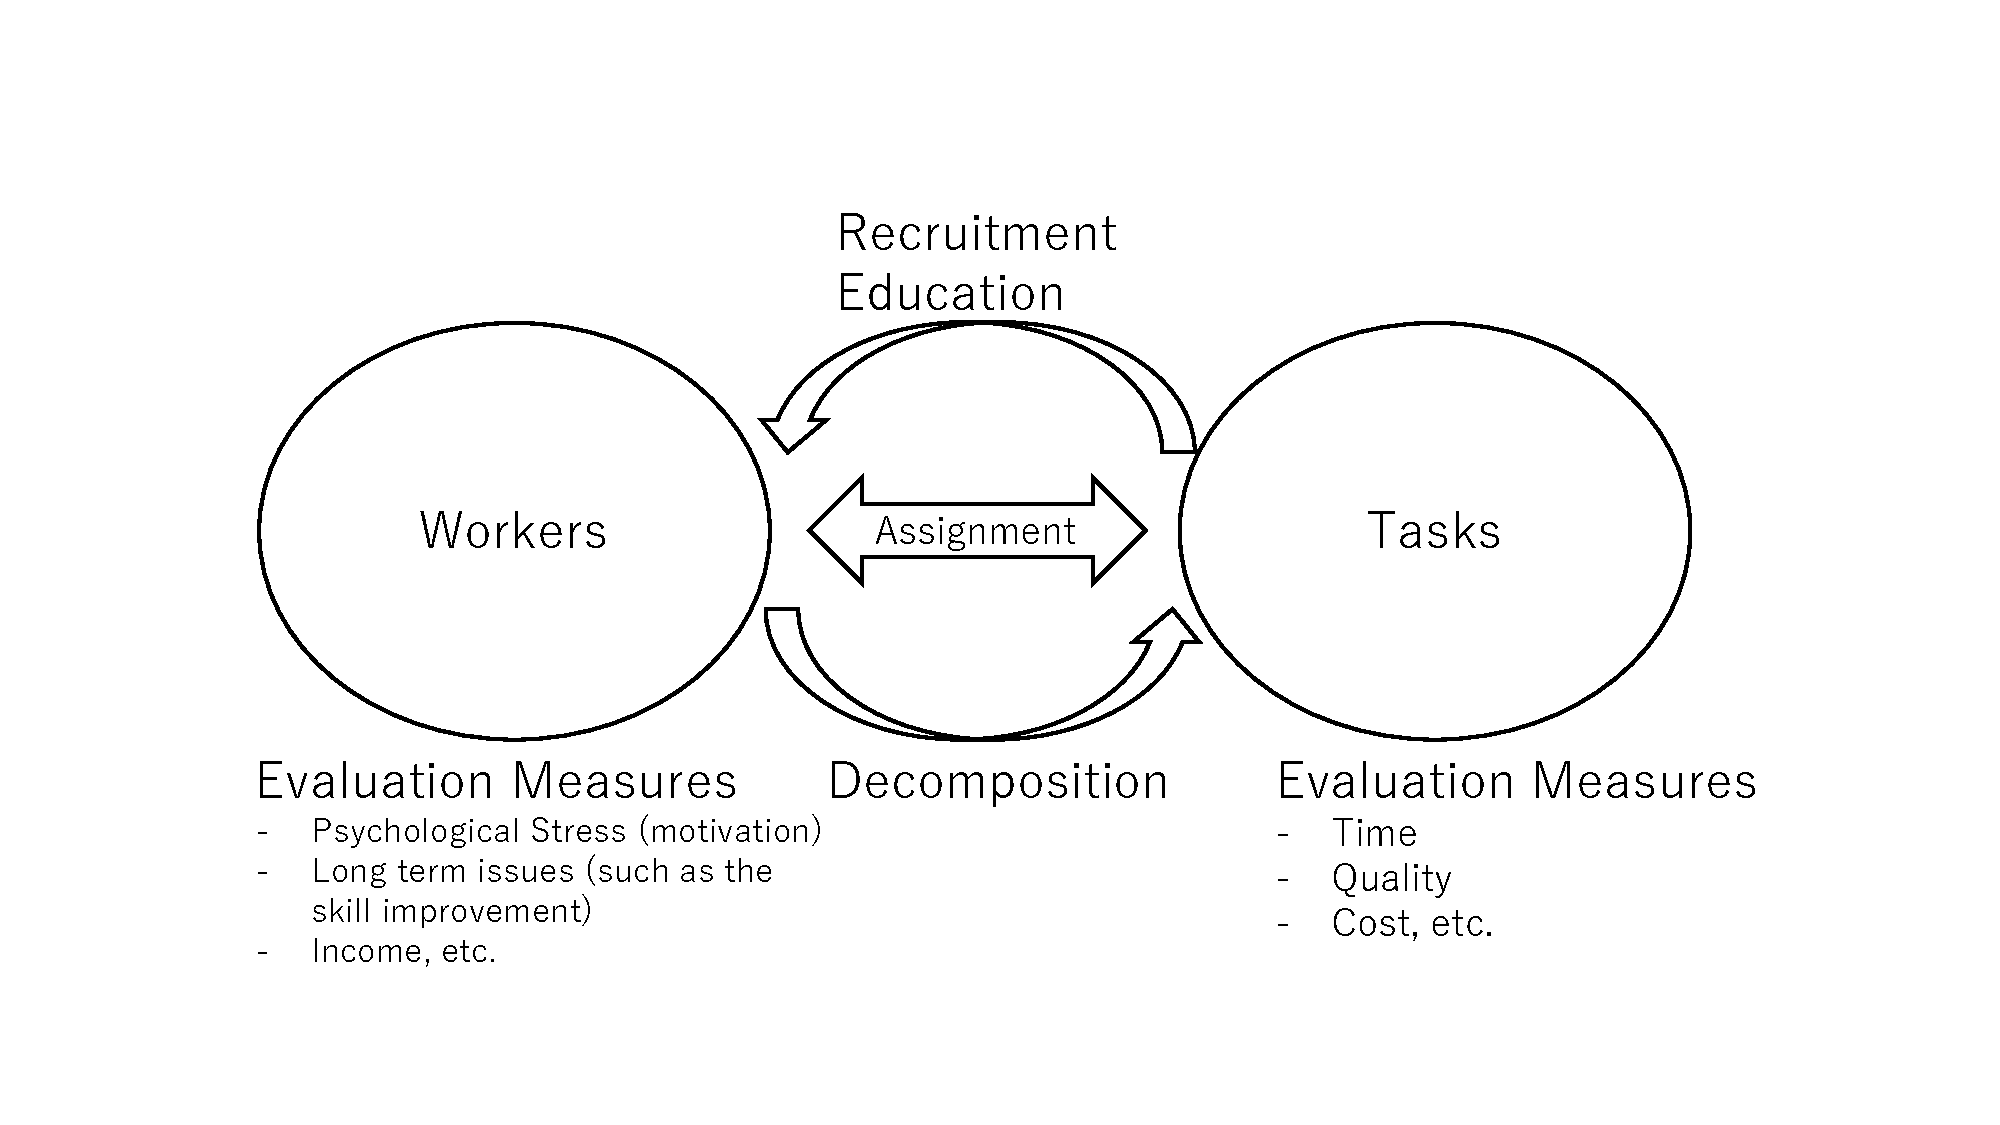
\includegraphics[width=.6\columnwidth]{figs/framework.pdf}
	\caption{System Overview}
	\label{fig:framwork}
\end{figure}
\fi
%%%%%%%%%%%%%%%%%%%%%%%%%%%%%%%%%%%%





